\documentclass{homework}

\newcommand{\hwname}{傅申}
\newcommand{\hwid}{PB20000051}
\newcommand{\hwtype}{人工智能基础}
\newcommand{\hwnum}{1}

\renewcommand{\questiontype}{3.}

\usepackage{verbatim}
\usepackage{listings}
\usepackage{tikz}
\usetikzlibrary{arrows.meta,automata,positioning}
\lstset{
    basicstyle=\ttfamily\small,
}

\begin{document}
\maketitle
\questionnumber{7}
\question{}
\begin{alphaparts}
    \questionpart{}
    \begin{description}
        \item[初始状态] 没有地区被染色的地图;
        \item[目标测试] 地图中所有地区都被染色, 且任何两个相邻的地区都没有染成相
            同的颜色;
        \item[后继函数] 为一个未被染色的区域染色, 且该颜色与该相邻区域的颜色不
            同;
        \item[耗散函数] 染色次数.
    \end{description}
    \questionpart{}
    \begin{description}
        \item[初始状态] 猴子和两个箱子均在屋子的地面上, 香蕉挂在房间的房顶上;
        \item[目标测试] 猴子拿到了香蕉;
        \item[后继函数] 移动, 爬上箱子, 爬下箱子, 移动箱子, 将一个箱子堆叠在另一
            个上, 拿取香蕉;
        \item[耗散函数] 操作次数.
    \end{description}
    \addtocounter{partCounter}{1}
    \questionpart{}
    \begin{description}
        \item[初始状态] 三个壶均为空;
        \item[目标测试] 某个壶中刚好有 1 加仑水;
        \item[后继函数] 装满某个壶, 倒空某个壶, 将某个壶中的水倒入另一个壶;
        \item[耗散函数] 操作次数.
    \end{description}
\end{alphaparts}

\questionnumber{9}
\question{}
\begin{alphaparts}
    \questionpart{}
    使用一个 3 元组描述状态, 其中三个元素分别代表原河岸的传教士, 野人和船的数目.
    显然元组 $(x, y, z)$ 满足 $0 \leqslant x, y \leqslant 3$, $z \in \{0, 1\}$.
    \begin{description}
        \item[初始状态] (3, 3, 1);
        \item[目标函数] (0, 0, 0);
        \item[后继函数] $actions: (x, y, z) \mapsto (x', y', z')$, 其中满足:
            \begin{itemize}
                \item $x' = y'$ 或 $x' = 0$ 或 $x' = 3$;
                \item $z + z' = 1$;
                \item 如果 $z = 1$ 则 $(x + y - x' - y') \in \{1, 2\}$, 否则
                      $(x' + y' - x - y) \in \{1, 2\}$;
                \item $(x - x') \times (y - y') \geqslant 0$;
            \end{itemize}
        \item[耗散函数] 每次操作代价均为 1.
    \end{description}
    按照上面的形式化描述, 完全状态空间图如下, 其中, 如果一个状态能转换到另一个状
    态, 则反之也成立, 故图中用双向箭头 $\leftrightarrow$ 代替两状态间相互转换的
    两个箭头以简化状态空间图. 箭头上的标识代表转换所对应的船上的传教士和野人人
    数.

    \begin{center}
        \resizebox{.9\textwidth}{!}{
            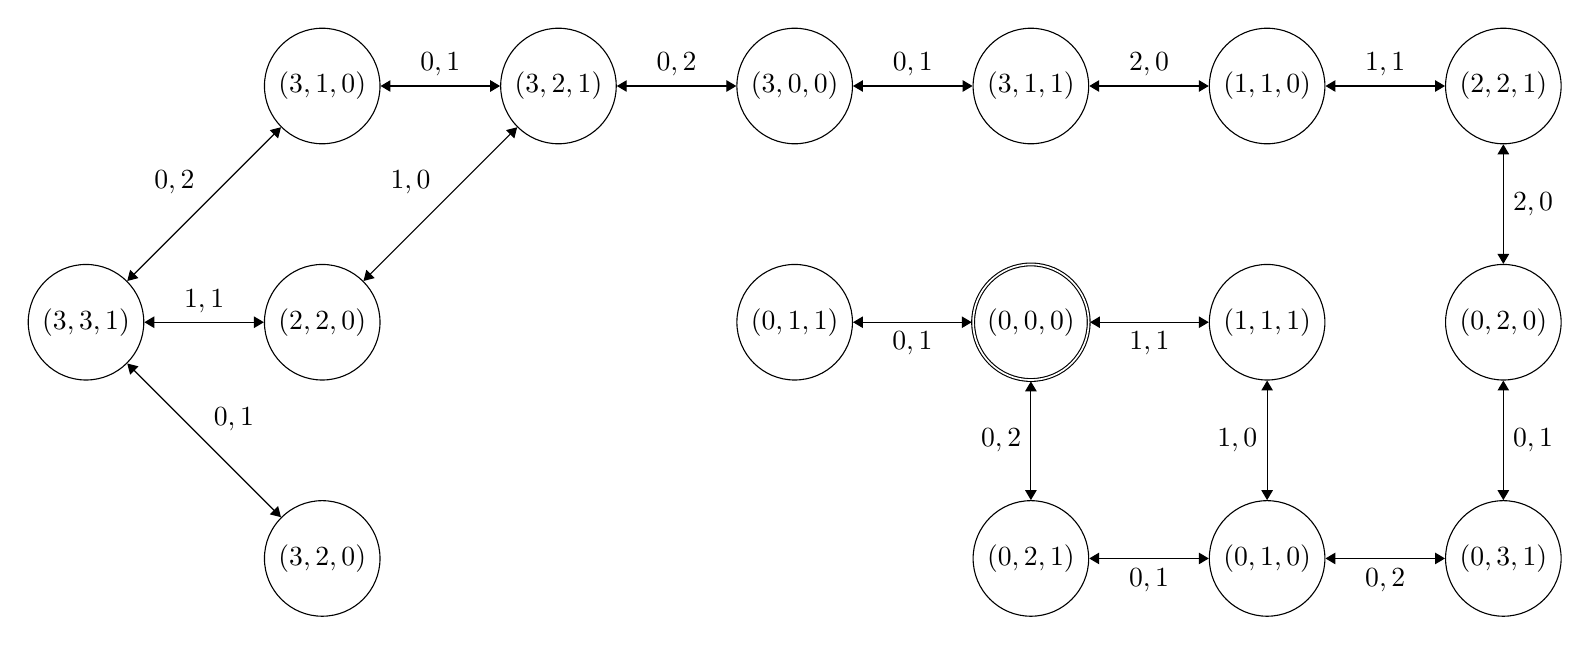
\begin{tikzpicture}[<->,>={Triangle},
                node distance=3cm, on grid, auto]
                \node [state]           (0)                {$(3, 3, 1)$};
                \node [state]           (1)  [right of=0]  {$(2, 2, 0)$};
                \node [state]           (2)  [above of=1]  {$(3, 1, 0)$};
                \node [state]           (3)  [below of=1]  {$(3, 2, 0)$};
                \node [state]           (4)  [right of=2]  {$(3, 2, 1)$};
                \node [state]           (5)  [right of=4]  {$(3, 0, 0)$};
                \node [state]           (6)  [right of=5]  {$(3, 1, 1)$};
                \node [state]           (7)  [right of=6]  {$(1, 1, 0)$};
                \node [state]           (8)  [right of=7]  {$(2, 2, 1)$};
                \node [state]           (9)  [below of=8]  {$(0, 2, 0)$};
                \node [state]           (10) [below of=9]  {$(0, 3, 1)$};
                \node [state]           (11) [left of=10]  {$(0, 1, 0)$};
                \node [state]           (12) [left of=11]  {$(0, 2, 1)$};
                \node [state]           (13) [above of=11] {$(1, 1, 1)$};
                \node [state,accepting] (14) [above of=12] {$(0, 0, 0)$};
                \node [state]           (15) [left of=14]  {$(0, 1, 1)$};

                \path
                (0)  edge node {$1, 1$} (1)
                (0)  edge node {$0, 2$} (2)
                (0)  edge node {$0, 1$} (3)
                (1)  edge node {$1, 0$} (4)
                (2)  edge node {$0, 1$} (4)
                (4)  edge node {$0, 2$} (5)
                (5)  edge node {$0, 1$} (6)
                (6)  edge node {$2, 0$} (7)
                (7)  edge node {$1, 1$} (8)
                (8)  edge node {$2, 0$} (9)
                (9)  edge node {$0, 1$} (10)
                (10) edge node {$0, 2$} (11)
                (11) edge node {$0, 1$} (12)
                (11) edge node {$1, 0$} (13)
                (12) edge node {$0, 2$} (14)
                (13) edge node {$1, 1$} (14)
                (14) edge node {$0, 1$} (15);
            \end{tikzpicture}
        }
    \end{center}
    \questionpart{}
    因为完全状态空间很小, 所以任何可获得最优解的搜索策略都是有效的, 比如 BFS,
    UCS, IDS 和双向搜索. 这里采用 BFS, 并且在扩张时不选择父节点和初始结点, 如下
    \begin{lstlisting}[language=Bash]
solve():
    frontier = Queue((3, 3, 1))
    while 
        if frontier.empty() then return failure
        head = frontier.dequeue()
        for state in succ(head) do
            if goal_test(state) then return the corresponding solution
            if state = (3, 3, 1) or state = head then continue
            frontier.enqueue(state)

goal_test((x, y, z)):
    return x = y = z = 0

succ((x, y, z)):
    actions = [(1, 1), (0, 2), (0, 1), (1, 0), (2, 0)]
    successors = []
    for (x, y) in actions do
        if z == 1 then
            successor = (x + y, x + y, 0)
            if is_valid(successor) then successors.append(successor)
        else
            successor = (x - y, x - y, 1)
            if is_valid(successor) then successors.append(successor)
    return successors

is_valid((x, y, z)):
    return 3 >= x, y >= 0 and (x = y or x = 0 or x = 3)
    \end{lstlisting}
    找到的一个可行的解为: $(3, 3, 1) \to (3, 1, 0) \to (3, 2, 1) \to (3, 0, 0)
        \to (3, 1, 1) \to (1, 1, 0) \to (2, 2, 1) \to (0, 2, 0) \to (0, 3, 1)
        \to (0, 1, 0) \to (1, 1, 1) \to (0, 0, 0)$.

    我认为检查重复状态是没有必要的, 因为虽然每条边都是双向的, 且完全状态空间中出
    现了环 (只出现在了初始结点和目标结点处), 但是这两种情况导致的重复遍历完全可
    以通过在扩张时不选择父节点和初始结点来避免.

    \questionpart{}
    可能的原因是人很难判断一个动作是否是有效的, 因为有效的动作需要满足的条件很
    多.
\end{alphaparts}
\end{document}
